\chapter*[Conclusion: Cosmology]{Conclusion: Cosmology}
\addcontentsline{toc}{chapter}{Conclusion: Cosmology}
\refstepcounter{chapter}

This part began by showing in Chapter~\ref{chap:kd} that almost all classical inflationary solutions begin in a generic kinetically dominated phase. The generality of this statement was discussed in Chapter~\ref{chap:kt}. 
Whether or not this phase occurs in reality can only be established by observation. If inflation was sufficiently short, then this pre-inflationary epoch may be observable as a suppression in power at low-$\ell$ in the $C_\ell$ spectrum, or in low-$k$ in the $\mathcal{P}_\mathcal{R}(k)$ spectrum. 

In Chapter~\ref{chap:rec}, I showed that if one reconstructs the primordial power spectrum $\mathcal{P}_\mathcal{R}(k)$ from a Bayesian perspective there is some weak evidence for a suppression of power at low-$k$, as well as an anomaly at $\ell\sim30$. Whilst this by no means provides evidence for an observable kinetically dominated epoch, it does suggest the possibility that with better data there could be.

In order to gain more theoretical guidance on the precise predictions which the kinetically dominated universe makes about the primordial power spectrum, we have to gain a greater understanding of the quantum mechanics of this phase. The details of this are non-trivial, since as soon as one migrates away from a de-Sitter limit, the theory as to how to set initial conditions becomes far more murky. Chapter~\ref{chap:qv} has enumerated some of these issues, and provided an alternative possibility for quantising a kinetically dominated universe.

\section*{Future work}
\subsection*{Theoretically investigating kinetically dominance}
The results of Chapter~\ref{chap:kt} require further investigation. In particular, since linear spatial perturbations grow backwards in time, the universe is more inhomogeneous closer to $t=0$. This will lead to a breakdown in the assumptions at some point, and it would be helpful to quantify this fully. In particular, it would useful to know if the breakdown is earlier than the Planck scale for $k$-scales of observational interest.

Further, since the kinetically dominated universe stabilises forwards in time, it would be interesting to quantify how generic our initial conditions are, and whether a homogeneous kinetically dominated phase naturally arises for any universe beginning with $\dot{\phi}^2\gg V(\phi)$. This would involve similar machinery to that used in ``eternal inflation'' scenarios.


\subsection*{Constraining the kinetically dominated universe}

The next task would be to ask if the data can provide any further insight into the quantum vacuum of the kinetically dominated universe. It would be particularly interesting to find out if the data themselves were capable of distinguishing between vacua. This could be done for the current set of cosmological data, or one could ask about the feasibility of future data sets in providing constraints on this portion of the unierse.

A full analysis would involve numerically integrating the quantum mechanical equations through the pre-inflationary phase all the way to horizon exit. Since these equations are highly oscillatory with time-varying coefficients, this would require a numerical method capable of tackling these. In fact, I have begun work on such a technique, which is detailed in Chapter~\ref{chap:RK}.

If one of these vacua is the ``correct'' one, it still remains to be determined when, if at all, it was in its vacuum state. It may be that we can provide observational constraints on the precise value of this moment.

\subsection*{Further constraints on inflation}
In addition, as a member of Planck core team II, I intend to continue more traditional observational reconstructions of inflationary and cosmological functions.

In general, inflationary analysis begins with the definition of the potential $V(\phi)$. This then predicts a primordial power spectrum $\mathcal{P}_\mathcal{R}(k)$ via a numerical integration of the Mukhanov-Sazaki (MS) equations. The primordial power spectrum is then converted via cosmological transfer functions ($\Delta$) into a set of multipole moments:

\tikzsetnextfilename{inflation_procedure}
\begin{center}
  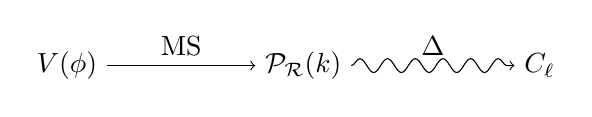
\begin{tikzpicture}[decoration=snake]
    \draw[] (3,0) node (Cl) {$C_\ell$};
    \draw[] (0,0) node (Pr) {$\mathcal{P}_\mathcal{R}(k)$};
    \draw[] (-3,0) node (Vphi) {$V(\phi)$};
    \draw[->,decorate] (Pr) -- (Cl) node[midway,above]{$\Delta$};
    \draw[->] (Vphi) -- (Pr) node[midway,above]{MS};
  \end{tikzpicture}
\end{center}

In Chapter~\ref{chap:rec} we applied a Bayesian reconstruction procedure to the middle stage, and reconstructed the primordial power spectrum in a model independent manner.  
We intend to apply our Bayesian reconstruction procedure separately to all three of these stages of the analysis, with the new updated polarisation data.
